\section{Historique}
%3
\begin{frame}
    \frametitle{L'évolution des cartes graphiques}
\begin{block}{Années 1980 : contrôleurs video}
  Ces circuits permettaient d'afficher sur un tube cathodique 
  des informations stockées en mémoire. Ils fournissaient des fonctionnalités de base, essentiellement orientées
  autour de la \bf{gestion de la mémoire vidéo} et de la génération des \bf{signaux de synchronisation}. 
  \begin{figure}[ht]
    \centering
    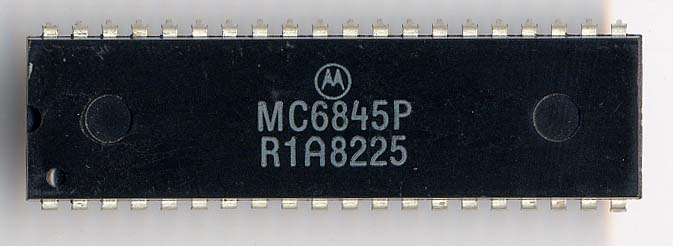
\includegraphics[scale=0.5]{Motorola_MC6845.jpg}
    \caption{Le contrôleur vidéo MC6845. \footnote{\tiny \url{https://commons.wikimedia.org/w/index.php?curid=976920}}}
    \label{fig:MC6845}
  \end{figure}
\end{block}
\end{frame}
%4
\begin{frame}
  \frametitle{L'évolution des cartes graphiques}
\begin{block}{Contrôleurs graphiques}
  Apparus vers la fin des années 1980, ils apportent des fonctionnalités graphiques, comme le \bf{tracé de segment}, 
  et gèrent une \bf{mémoire distincte} de celle de l'unité centrale.
   \begin{figure}[htbp]
    \centering
    \hfill
   \begin{subfigure}{0.4\textwidth}
    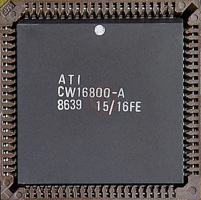
\includegraphics[scale=0.45]{ATI16800.jpg}
   \end{subfigure} 
   \hfill
   \begin{subfigure}{0.4\textwidth}
    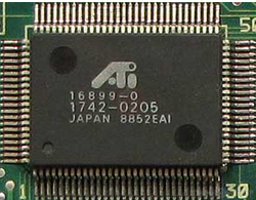
\includegraphics[scale=0.45]{ATI16899.jpg}
   \end{subfigure} 
   \hfill
    \caption{Contrôleurs graphiques.}
    \label{fig:graphic_controllers}
   \end{figure}
\end{block}
\end{frame}
%5
\begin{frame}
  \frametitle{L'évolution des cartes graphiques}
\begin{block}{Les processeurs graphiques 3D.}
    Disponibles pour le grand public depuis le milieu des années 1990, ils incluent des fonctionnalités
    d'affichage en trois dimensions. Parallèlement, des bibliothèques logicielles font leur apparition
    (OpenGL, Direct3D). L'affichage d'\bf{une scène} est réalisé à travers un \bf{pipeline graphique}~: 
        
        \begin{enumerate}
            \item transformation de sommets;
            \item projection;
            \item traçage.
        \end{enumerate}
    
    \begin{figure}[htbp]
        \centering
       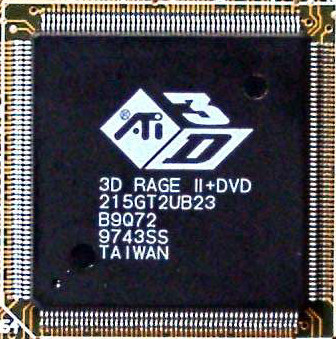
\includegraphics[scale=0.15]{3drage.jpg} 
        \caption{Contrôleur 3D ATI Rage.}
        \label{fig:ati_rage}
    \end{figure}
\end{block}
\end{frame}

\begin{frame}
  \frametitle{L'évolution des cartes graphiques}
\begin{block}{Les premiers pas du pipeline graphique.}
    \begin{figure}[htbp]
        \centering
       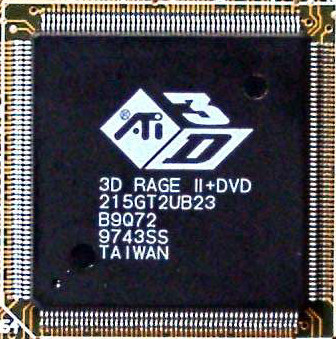
\includegraphics[scale=0.15]{3drage.jpg} 
        \caption{Contrôleur 3D ATI Rage.}
        \label{fig:ati_rage}
    \end{figure}
\end{block}
\end{frame}


%6
\begin{frame}
  \frametitle{L'évolution des cartes graphiques}
\begin{block}{Les processeurs progammables}
    En 2001, la société NVIDIA introduit sur le marché les processeurs graphiques
    GeForce 3 qui permettent de programmer les étapes du pipeline graphique. 
    \begin{figure}[htbp]
        \centering
       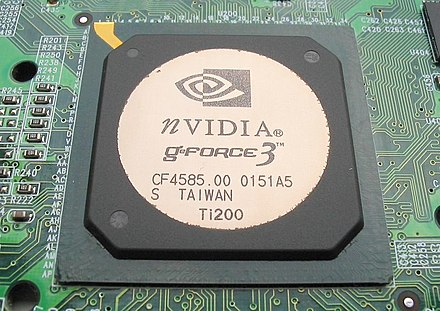
\includegraphics[scale=0.25]{Geforce3gpu.jpg} 
        \caption{Contrôleur 3D programmable.}
        \label{fig:geforce3}
    \end{figure}
\end{block}
%7
\end{frame}

\begin{frame}
  \frametitle{L'évolution des cartes graphiques}
\begin{block}{Le calcul}
    Fin 2006, NVIDIA introduit l'environnement de développement CUDA qui
    permet d'exploiter la puissance de calcul des cartes graphiques pour des applications générales.
    Les performances théoriques sont comparables à celles d' un 
    superordinateur, mais  pour une enveloppe énergétique et un coût bien inférieurs.

    \begin{figure}[htbp]
        \centering
       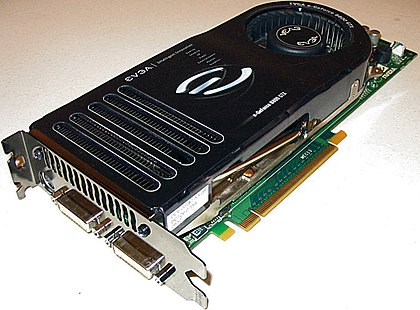
\includegraphics[scale=0.2]{geforce8800.jpg} 
        \caption{Carte graphique CUDA.}
        \label{fig:gforce8}
    \end{figure}
\end{block}
\end{frame}

\begin{frame}
  \frametitle{Synthèse de l'évolution des cartes NVIDIA}
\begin{table}
\footnotesize  \centering
            \begin{tabular}{cccccc}
            \rowcolor{lightgray}\textbf{Année} & \textbf{Carte} & \textbf{Architecture} & \textbf{Cœurs\footnote{\tiny Cœurs \bf{CUDA} qui n'est pas la même notion qu'un coeur CPU !}}} & \textbf{RAM} & \textbf{Puissance} \\\hline
            1995 & NV1 & Dizaines de µm & ?  & 4 Mo & 2 Watts \\
            ... & ... & ...  & ... & ... & ...\\
    
            2017 & GTX 1080 Ti & Volta 16 nm & 3584 & 11 Go & 257 W \\
            2019 & GTX 2080 Ti & Turing 12 nm & 4352 & 11 Go & 290 W \\
            2020 & RTX 3090 & Ampere 8 nm & 10 496 & 24 Go & 350 W \\

            2022 & RTX 4090 & Ada Lovelace 5 nm & 18 000  & 24 Go & 450-600 W \\ 
            \end{tabular}
          \caption{Évolution des cartes NVIDIA.}\label{tab:evo_nvidia}
          \end{table}
\end{frame}
